\section{Méthodes d'évaluation}

Pour évaluer l'application, nous allons réaliser une étude dans laquelle on modifie deux facteurs, la présence ou non de la stimulation tactile et la présence ou non de la modification du corps. La raison pour laquelle nous modifions ces deux facteurs est que nous voulons tester l'impact de ces deux paramètres et pour cela, il nous faut des conditions permettant d'obtenir des mesures de contrôle afin d'obtenir une base pour comparer les résultats. Ceci nous donne les quatre conditions suivantes :
\begin{itemize}
\item Condition 1 : Le bâton virtuel se déplace automatiquement, le sujet n'est pas touché par le bâton réel. Le corps n'est pas modifié.
\item Condition 2 : Le bâton virtuel se déplace automatiquement, le sujet n'est pas touché par le bâton réel. Le corps est modifié.
\item Condition 3 : Le sujet est touché par le bâton réel et le bâton virtuel reproduit les mouvements du bâton réel. Le corps n'est pas modifié.
\item Condition 4 : Le sujet est touché par le bâton réel et le bâton virtuel reproduit les mouvements du bâton réel. Le corps est modifié.
\end{itemize}
Pour chaque conditions, la durée d'utilisation de l'application est de 60 secondes. Les différences entre les conditions 1 et 2 et les conditions 3 et 4, permettent d'obtenir des résultats pour voir l'influence de la modification du personnage. Dans les deux premières conditions, le bâton virtuel est présent mais il bouge automatiquement et le sujet n'est pas touché par le vrai bâton en même temps. Dans ces deux conditions, le sujet voit son avatar être touché par un bâton virtuel au niveau du dos avec des mouvements de haut en bas. Alors que dans les deux dernières conditions, le bâton virtuel reprend les mouvements du bâton réel et le sujet est donc touché par le bâton en même temps que son avatar (Voir Figure \ref{batonAvatarS}). Les différences entre les deux premières conditions et les deux dernières conditions, permettent de voir le réel impact du bâton virtuel qui reprend les mouvements du bâton réel et qui permet de créer la sensation de sortie de corps en réalité virtuelle.\\

Chaque sujets utilisent l'application suivant les quatre conditions. Entre chaque conditions, leur capacité à se localiser dans l'espace et leur perception de la largeur de leur corps sont mesurées et un questionnaire leur est donné. Durant l'expérience et les mesures, les participants portent un casque de réalité virtuelle \emph{Oculus Rift DK2} et un casque audio pour ne pas être dérangé par les bruits extérieurs. Tout d'abord, le sujet choisi l'avatar qui lui est le plus proche en terme de corpulence puis l'expérimentateur choisi un autre avatar. Ensuite, un premier essai est réalisé, dans le but de présenter l'expérience, où les participants peuvent tester l'application en bougeant leur avatar et voir le bâton virtuel, ainsi que pour montrer comment sont réalisées les mesures. On profitent de cette session d'entrainement pour obtenir les valeurs de comparaison pour chaque mesures. Afin que nos mesures ne soit pas faussées par le fait que le sujet peut s'habituer à l'exercice, particulièrement pour la localisation dans l'espace, les conditions peuvent être faites dans deux ordres différents : 1,2,3,4 et 3,4,1,2. Ainsi, on peut savoir si ce sont réellement les conditions qui impactent les résultats obtenus.
\begin{figure}[!h]
   	\centerline{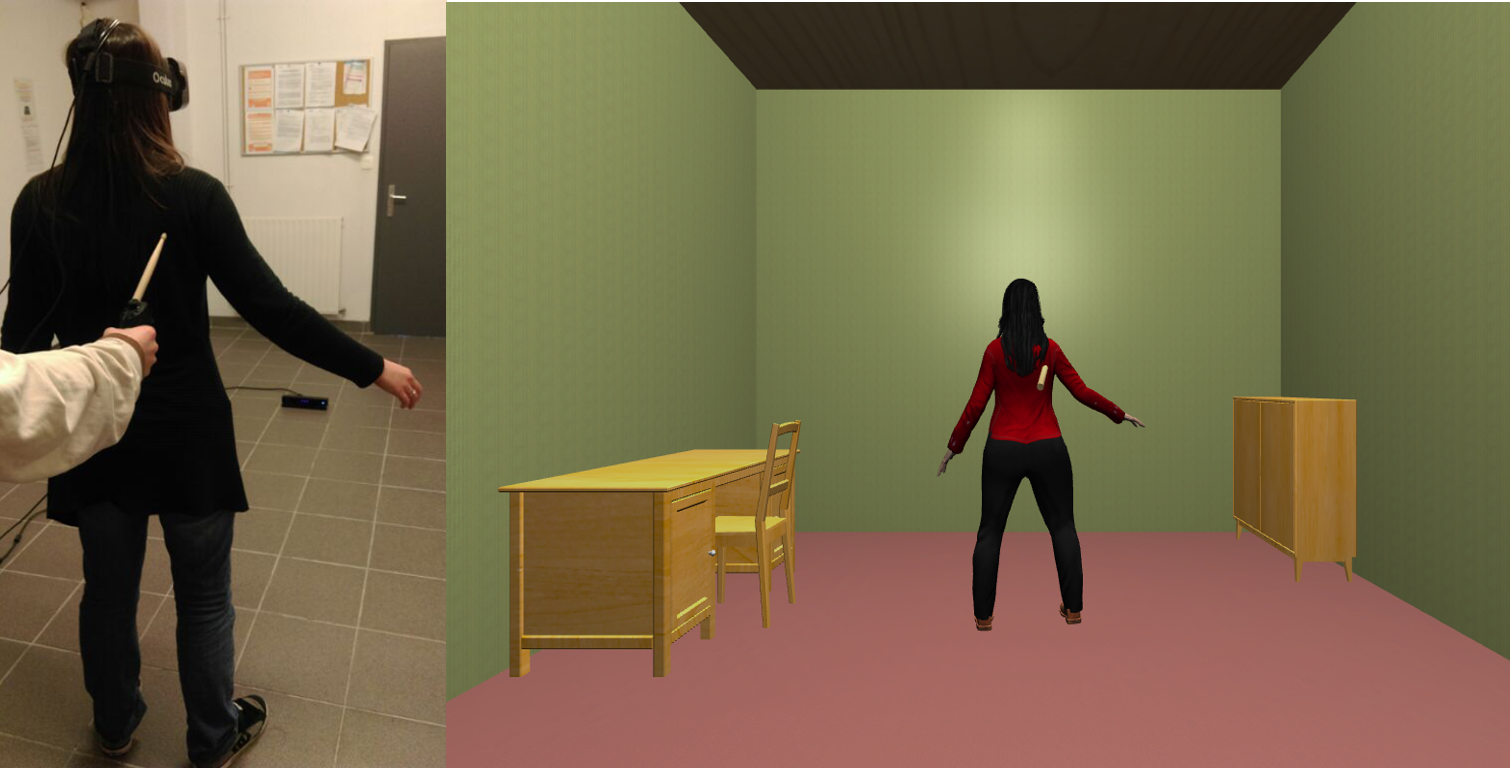
\includegraphics[scale=0.35]{images/doubleView2}}
   	\caption{\label{batonAvatarS} Utilisateur et avatar touchés par le bâton }
\end{figure}
\subsection{Localisation dans l'espace}
Pour mesurer la capacité à se localiser dans l'espace, le sujet doit marcher sur place pendant que l'expérimentateur le recule d'une distance constante entre chaque essai. On demande ensuite au participant de se replacer là où il était. Durant toute cette mesure, le sujet garde le casque et ne vois donc pas devant lui. On mesure ensuite la distance entre l'endroit où le sujet se replace et l'endroit où il était réellement. Pour cette mesure, on s'inspire de celle réalisée par Blank et al. \cite{bl10} dont le but est d'évaluer objectivement si le sujet à ressenti une illusion de sortie de corps.
\subsection{Perception de la largeur du corps}
\begin{figure}[!h]
   	\centerline{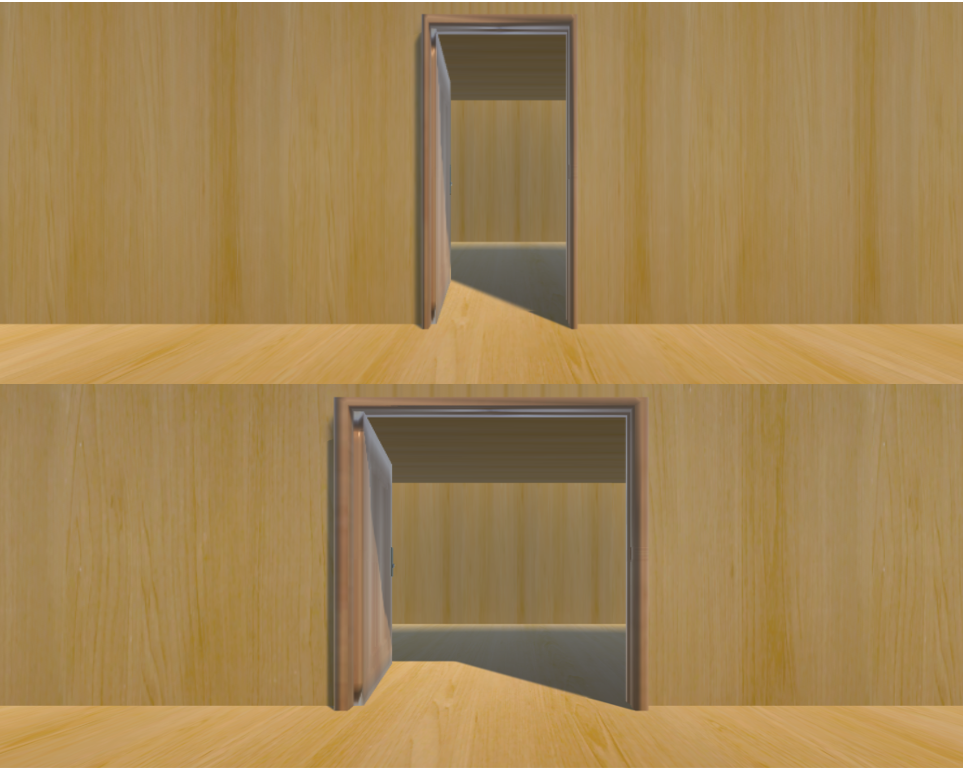
\includegraphics[scale=0.25]{images/doubleDoor3}}
   	\caption{\label{figDoor} Deux portes de largeur différentes }
\end{figure}
Pour connaître la perception implicite que le sujet a de la largeur de son corps, on réalise une mesure proche de celle faite par Guardia et al. \cite{gu10}. Le sujet voit via son casque de réalité virtuelle une série de trente portes qui peuvent avoir six largeurs différentes (Voir Figure \ref{figDoor}). Ainsi le sujet voit à cinq reprise chaque différente porte, et on s'assure que la même porte n'est pas affiché deux fois de suite. Pour chaque porte, le sujet doit dire si il peut passer à travers la porte sans avoir besoin de tourner les épaules. l'ordre des portes est aléatoire et donc différent à chaque mesure.

\subsection{Questionnaire}
Nous avons créés plusieurs questionnaires en fonction des conditions de l'expérimentation. Les participants doivent répondre à chaque question en utilisant une échelle à sept valeurs allant de -3 à 3, avec 3 signifiant 'pas du tout d'accord' et 3 'tout à fait d'accord'. Pour l'élaboration de nos questionnaires, nous nous somme inspirés de ceux fait dans d'autre étude sur la sortie de corps comme Lenggenhager et al. \cite{le07} auxquelles, nous avons rajouter d'autres questions plus spécifiques à notre expérience.Dans le questionnaire pour les conditions 3 et 4 (Voir Annexe \ref{questionnaires2}), trois questions ont pour but de mesurer la sortie de corps selon le ressenti du sujet :
\begin{itemize}
\item Q1 : j'ai eu l'impression de me sentir touché(e) au même endroit qu'était touché le corps virtuel par le bâton.
\item Q2 : j'ai eu l'impression que la sensation d'être touché(e) a été causée par le bâton qui touché le corps virtuel.
\item Q3 : j'ai eu la sensation que le corps virtuel était mon corps.
\end{itemize}

On ajoute d'autres questions, notamment une qui permet d'avoir le retour sur la synchronisation entre réel et virtuel pour le bâton, et deux autres dont on pourra voir si les résultats seront en corrélation avec les résultats de la localisation dans l'espace : 
\begin{itemize}
\item Q4 : j'ai eu l'impression que mon corps (réel) a dérivé vers l'avant (vers le corps virtuel).
\item Q7 : il m'a semblait que visuellement le corps virtuel a dérivé vers l'arrière (vers le corps réel).
\end{itemize}
Ainsi, si dans la mesure de la localisation dans l'espace, le sujet se replace moins loin ou plus loin de là où il se trouvait réellement, on pourra voir si cela se reflète dans ces réponses ou inversement. Pour le questionnaire des conditions 1 et 2 (Voir Annexe \ref{questionnaires1}), on retrouve les même questions que dans le questionnaire décrit précédemment sans celle sur la synchronisation du bâton et la Q2. car dans ces conditions il n'y a pas de bâton réel qui touche le sujet. On garde les questions Q1. et Q3. car cela nous permet d'avoir une base de comparaison pour voir l'effet lorsque le bâton réel et virtuel font les même mouvements.\\

Le questionnaire de fin (Voir Annexe \ref{questionnaires3}) permet d'obtenir des informations en ce qui concerne l'habitude des participants à interagir avec un environnement virtuel. Il permet également de recueillir des retours sur la qualité de l'application en ce qui concerne l'apparence de l'avatar, réalisme et aussi si il y avait une vrai impression de ressemblance pour la corpulence, et également pour tout ce qui concerne la capture du mouvement que ce soit pour l'avatar ou pour le bâton. Ces informations supplémentaire pourront nous aider à voir l'impact des aspects techniques mis en place sur les résultats obtenus.


